\chapter{Layered Entrepreneurial Leverage in San Antonio}

This lecture gives us no boardwork to reproduce, so we proceed in a different but still disciplined way. We follow the spoken order closely, because the order itself carries the argument: first visible scale, then the control law for growth, then the role of daily conduct, then perseverance, then capital allocation, then the long discipline of craft, and finally the stacked economics of property and transport. To keep the quantitative claims clear, we use light bookkeeping notation for gross income, net worth, and time scale, while treating all arithmetic as transcript-led and keeping explicit note of what is only a cautious reconstruction.

\section{Opening Benchmarks: Wealth Before Method}

The lecture opens by showing us outcome before mechanism. A flashy teaser around a high-end car, later clearly the Audi R8, is followed almost immediately by the question: what was the most amount of money made in a single year? The first purpose is not explanation. It is calibration.

\begin{definition}
We write \(G\) for gross revenue or income, \(NW\) for net worth, and use subscripts \(y\), \(m\), and \(d\) for yearly, monthly, and daily time scales. This is bookkeeping notation for the notes, not notation spoken in the interview.
\end{definition}

The first opening scale markers are therefore
\begin{equation}
G_{y,\max}^{\mathrm{early}}
\in
\{\$1{,}000{,}000,\;>\$500{,}000\}.
\end{equation}

The lecturer then states the governing question of the video: not only how these people became wealthy, but how one might begin a path toward wealth now. That sentence matters. It tells us how to read the rest of the chapter. Each interview is not a separate profile. Each one is a partial answer to a single problem: how earnings, discipline, capital, and leverage are made to work together.

\section{Crawl, Walk, Run: The First Control Law}

The first substantial respondent has worked in several roles: wealth management, corporate leadership, and construction. The interviewer asks what was implemented in order to scale businesses, and the answer comes back in the simplest possible form:
\begin{equation}
\text{crawl} \longrightarrow \text{walk} \longrightarrow \text{run}.
\end{equation}

\paragraph{Anecdote.}
The speaker does not celebrate instant scale. He warns that going all out from the start makes it impossible to recover when something goes wrong.

\paragraph{Claim.}
Growth has a correct order. If we enlarge the business faster than we enlarge our understanding, then leverage ceases to be an amplifier and becomes a failure mechanism.

\paragraph{Mechanism.}
The warning in the transcript is specific: run too fast and one over-leverages; over-leverage means too much debt; too much debt means a small mistake becomes unrecoverable. The antidote is not timidity. It is staged competence.

\subsection{Question \& Answer}

\paragraph{Question.}
How do we scale without breaking the business?

\paragraph{Answer.}
The lecture's answer is to control the step size. We first build a model that can survive a modest error, then a model that can survive a larger one, and only then a model that can carry serious leverage. In business language, expertise must precede acceleration. Debt should come after resilience, not before it.

This first answer does more than solve a local problem. It sets the rhythm for the rest of the lecture. Every later success story is to be measured against the same standard: does scale come after learning, or before it?

\section{Personal Stability and the Daily Resume}

The lecture now makes a turn that would be easy to underestimate. The same respondent is asked for the best financial decision of his career, and the answer is marriage. Then the advice to a younger self becomes: every day is an interview; every day is your resume.

\paragraph{Anecdote.}
A happy personal life is said to be necessary for success in business life. If it is all business, one will not be happy in the end.

\paragraph{Claim.}
The lecture is broadening the causal field. Business success is not treated as a narrow function of deals alone. Character, attitude, conduct, and personal steadiness enter the picture as economic inputs.

\paragraph{Mechanism.}
A compact editorial summary of the spoken logic is
\begin{equation}
\text{daily conduct}
\longrightarrow
\text{reputation}
\longrightarrow
\text{future opportunities}.
\end{equation}
This is not a spoken formula, but it preserves the point faithfully. We are not judged only in formal interviews. We are judged in repeated contact, under ordinary conditions, by how we carry ourselves when the stakes seem low.

The lecture then pauses for a caricature intermission. That pause is not accidental. It resets the pace, and when the chapter resumes we are no longer in the world of life-structure alone. We are back in entrepreneurship proper, now with a founder who has sold a company.

\section{Perseverance, Friction, and the AI Pivot}

A founder from bioinformatics appears next. The field is described as computer science and medical school combined. He has sold a business, although he does not disclose the sale price. The interviewer then asks for advice to someone starting a business in the present moment.

\paragraph{Anecdote.}
The answer is that perseverance is one of the most underappreciated aspects of business. The founder insists that friction is universal and that the people who make it are the ones who stay with the problem.

\paragraph{Claim.}
Growth does not happen in a frictionless environment. It happens because the business survives its friction. Adversity is not an accidental side effect. It is part of the medium through which entrepreneurs move.

\subsection{Question \& Answer}

\paragraph{Question.}
What matters most when the business looks as if it may fail?

\paragraph{Answer.}
The lecture answers with perseverance, but not in a vague sense. One must believe in the business and in the team's ability to cross the bad interval rather than surrender to it. Growth comes from friction only if one remains present long enough to extract the lesson from it.

The next question changes scale again. What industry should people look to enter now? The answer is AI, and the lecture is careful about what this means. The point is not that machines replace all jobs automatically. The sharper claim is that the worker who learns to use AI well can replace the worker who does not.

In that spirit, the lecture pivots again. We have heard about growth discipline, character, and perseverance. We now move to capital allocation: given earnings, where should they go?

\section{Land, Craft, and the Shape of a Working Life}

The lecture relocates to the hotel and begins again with scale markers. Another respondent reports about a million dollars as the most ever made in a year and a net worth on the order of
\begin{equation}
NW \approx \$15\text{M}--\$20\text{M}.
\end{equation}
The interviewer then asks where people should invest when they begin to make money.

\paragraph{Anecdote.}
The answer is land. The argument is concrete: they are not making more of it; development costs keep rising; land can always be used for something; agricultural use can keep taxes low; later development and sale can generate both return and capital gains.

\paragraph{Claim.}
The lecture's capital-allocation point is that scarce, reusable assets can be superior stores and multipliers of earnings.

\paragraph{Mechanism.}
As a compact shorthand for the transcript, we may write
\begin{equation}
\dot S_{\mathrm{land}} \approx 0,
\qquad
\dot C_{\mathrm{develop}} > 0,
\end{equation}
where \(S_{\mathrm{land}}\) stands for effective supply and \(C_{\mathrm{develop}}\) for development cost. This is not lecture notation. It is a note-taking device. The point is that fixed supply combined with rising development cost creates option value for the landholder.

\subsection{Question \& Answer}

\paragraph{Question.}
Where should earned money go if we want it to multiply?

\paragraph{Answer.}
One answer offered by the lecture is land: low current tax burden under some uses, later development, and eventual capital gains. But the lecture refuses to let that become the only answer. Immediately after the real-estate developer, it widens the frame and reminds us that not every path to high income looks like large-scale property development.

We return to the caricature artist. He has been drawing for about \(35\) years, says that people from all over are friendly and curious to see themselves in caricature form, and reports a top annual income in the range
\begin{equation}
G_{y,\max}^{\mathrm{artist}} \approx \$300{,}000\text{--}\$400{,}000.
\end{equation}
He also says that he has drawn almost half a million people. The importance of this section is not merely the figure. It is that long practice in a visible craft can itself become a durable economic machine.

The architect who follows sharpens the point further. She owns her practice, works for herself, and gives financial advice that is not about one asset class or one industry. It is about destiny, choices, and the lifestyle one wants to live. The lecture thereby inserts a hidden variable into the economics: it is not enough to maximize a number if the life built around the number is not one we want to inhabit.

By the end of this stretch we have been shown three different mechanisms of durable value: scarcity in land, long practice in craft, and self-direction in professional work. Only now does the lecture return to the man from the opening teaser and begin the most explicit case study in repeatable enterprise.

\section{The First Property: Research, Duplication, and Portfolio Scale}

The speaker now returns to the man associated with the R8. We are told that real estate was the first large investment, that the biggest year was about \(\$1.3\) million gross total, and that the combined total of units and properties is about \(38\text{--}40\).

\paragraph{Anecdote.}
The interviewer's question is how someone really starts a path to becoming wealthy. The answer begins not with a tactic but with orientation: find something one is truly willing to go hard at, then invest in it, learn everything around it, and duplicate the deal structure.

\paragraph{Claim.}
What the lecture is now trying to establish is that scale need not come from novelty. It can come from repetition. We do not need a fresh invention at every step. We need a model that can be learned, executed, and replicated.

\paragraph{Mechanism.}
The main portfolio data may be written as
\begin{equation}
N_{\mathrm{holdings}} \approx 38\text{--}40,
\qquad
G_{\mathrm{portfolio},y} \approx \$1.3\times 10^6 \ \text{gross}.
\end{equation}

The lecture also gives us a behavioral modifier: staying humble. Humility is important here not as etiquette but as an operating condition for learning. Once we think we know enough, growth stops because observation stops.

\subsection{Question \& Answer}

\paragraph{Question.}
If we had zero properties and zero rentals, what is the first move toward the first deal?

\paragraph{Answer.}
The lecture's answer is research, and it is more concrete than the word sometimes suggests. Research means looking at the city, the specific area, the platform itself, and the offerings already succeeding there. One studies the existing pattern before placing the first bet.

A narrow, transcript-derived schematic is useful here:

\begin{figure}[t]
\centering
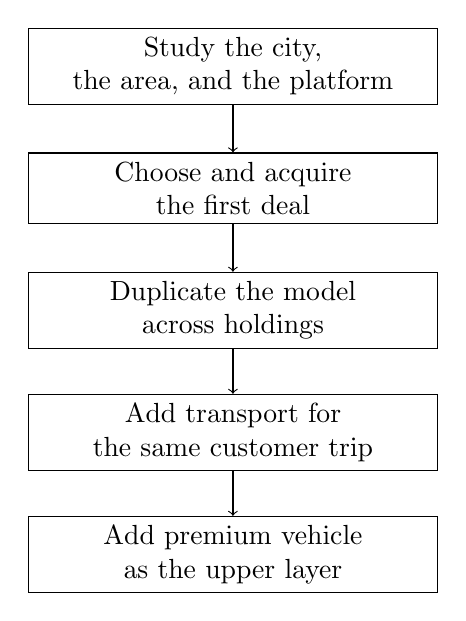
\begin{tikzpicture}[x=1cm,y=1cm]
\node[draw,align=center,minimum width=5.2cm,minimum height=0.85cm] (a) at (0,0) {Study the city,\\the area, and the platform};
\node[draw,align=center,minimum width=5.2cm,minimum height=0.85cm] (b) at (0,-1.55) {Choose and acquire\\the first deal};
\node[draw,align=center,minimum width=5.2cm,minimum height=0.85cm] (c) at (0,-3.10) {Duplicate the model\\across holdings};
\node[draw,align=center,minimum width=5.2cm,minimum height=0.85cm] (d) at (0,-4.65) {Add transport for\\the same customer trip};
\node[draw,align=center,minimum width=5.2cm,minimum height=0.85cm] (e) at (0,-6.20) {Add premium vehicle\\as the upper layer};
\draw[->] (a) -- (b);
\draw[->] (b) -- (c);
\draw[->] (c) -- (d);
\draw[->] (d) -- (e);
\end{tikzpicture}
\caption{A transcript-derived ladder of leverage. The lecture moves from research to the first property, then to duplication, then to adjacent services built around the same trip.}
\end{figure}

The quantitative example now becomes useful. The speaker says that one property can gross about \(\$3{,}000\text{--}\$5{,}500\) per month. Let us annualize that carefully:
\begin{align}
G_{\mathrm{property},y}
&= 12\,G_{\mathrm{property},m} \\
&\approx 12 \times (\$3{,}000\text{--}\$5{,}500) \\
&\approx \$36{,}000\text{--}\$66{,}000.
\end{align}

We may also compute a rough portfolio-wide average per holding:
\begin{align}
\bar G_{\mathrm{holding},y}
&= \frac{G_{\mathrm{portfolio},y}}{N_{\mathrm{holdings}}} \\
&\approx \frac{\$1.3\times 10^6}{38\text{--}40} \\
&\approx \$32{,}500\text{--}\$34{,}200,
\end{align}
and hence
\begin{equation}
\bar G_{\mathrm{holding},m}
=
\frac{\bar G_{\mathrm{holding},y}}{12}
\approx \$2.7\text{k}\text{--}\$2.85\text{k}.
\end{equation}

We should read these numbers cautiously. The holding count mixes units and properties, and the \(\$1.3\) million is given as gross total, so the average is only a rough orientation. Still, the arithmetic does exactly what the lecture wants it to do: it shows how duplication turns a moderate unit-level gross into a large aggregate total.

\section{Layered Enterprise: Turo, the R8, and the Second Revenue Layer}

The last movement is the lecture's clearest piece of entrepreneurial engineering. The property business is already working. Guests book places to stay. Once that is true, another need appears automatically: they must move around. The second business is therefore not random diversification; it is the monetization of the next need in the same trip.

\paragraph{Anecdote.}
The speaker explains that the car business grew out of the property business. Guests who booked lodging also needed transportation. Regular vehicles came first; exotic vehicles followed as a premium layer. Turo is described as the Airbnb for cars.

\paragraph{Claim.}
The major claim here is that adjacent services can be stacked on top of one another when they are driven by the same customer event.

\paragraph{Mechanism.}
A simple bookkeeping identity expresses the logic:
\begin{equation}
R_{\mathrm{trip}}
=
R_{\mathrm{lodging}}
+
R_{\mathrm{transport}}
+
R_{\mathrm{premium}}.
\end{equation}
This is not the speaker's notation, but it is the cleanest way to preserve his point. The same traveler can support multiple streams of gross revenue.

The lecture now gives us its sharpest operating numbers. Some cars, we are told, can do about \(\$8{,}000\text{--}\$10{,}000\) per month, and the R8 typically goes for about \(\$600\text{--}\$700\) a day. We therefore write
\begin{equation}
G_{R8,m}=p_{R8,d}\,d_{R8,m},
\qquad
p_{R8,d}\approx \$600\text{--}\$700.
\end{equation}

This lets us perform a cautious consistency check. If we use the monthly gross figure only as an order-of-magnitude benchmark for a premium car, then the booked days per month would satisfy
\begin{align}
d_{R8,m}
&= \frac{G_{R8,m}}{p_{R8,d}} \\
&\approx \frac{\$8{,}000\text{--}\$10{,}000}{\$700\text{--}\$600} \\
&\approx 11.4\text{--}16.7
\quad
\text{booked days per month}.
\end{align}

\begin{remark}
This should not be overstated. The transcript says that \(\$8{,}000\text{--}\$10{,}000\) can happen on some cars, not necessarily that the R8 itself always realizes that number. The calculation is therefore a plausibility check, not a proof.
\end{remark}

Still, the result is illuminating. At a daily rate of roughly \(\$600\text{--}\$700\), meaningful monthly gross does not require perfect occupancy. It requires a premium asset with enough demand concentration, especially around weekends and visitor traffic, to convert a relatively small number of bookings into a serious line of revenue.

\subsection{Question \& Answer}

\paragraph{Question.}
How do we add a second revenue layer without starting from scratch?

\paragraph{Answer.}
We follow the first customer's next need. Property guests need transportation. Transportation can be offered in ordinary form or premium form. The new business therefore does not stand alone. It stands on top of the first business and deepens the amount extracted from the same trip.

The final question of the lecture asks how someone should start in exotic car rental. The answer returns us, fittingly, to the lecture's first law: structure first, acceleration later. Form the LLC, learn how to hold the vehicles inside it, build business credit where needed, and add this layer most effectively when something underneath it is already working.

\section{Summary}

The lecture begins with spectacle and ends with structure. We are first shown million-dollar years and a luxury car, but the real content unfolds slowly: scale must be staged; debt must not outrun competence; private stability supports public success; perseverance matters because friction is unavoidable; land can multiply earnings through scarcity and development option value; craft and self-owned professional work remain serious economic paths; research precedes the first deal; duplication creates portfolio scale; and the strongest enterprises often grow by layering adjacent services around the same customer.

What finally emerges is a compact model of entrepreneurial leverage. The first layer is discipline and judgment. The second is a repeatable asset or operating system. The third is adjacent monetization. In the language of the lecture, we do not become wealthy merely by moving faster. We become wealthy by learning what can be repeated, what can be owned, and what can be added on top once the first layer is already in motion.